\section{Introduction of the Physical Problem}
    \begin{frame}[t]
        \frametitle{Particle Types}
        
        \vspace{-0.4cm}

        \begin{minipage}[t]{0.5\textwidth}
            \vspace{0pt}
            \begin{itemize}
                \item Bosonic operators \pause
                \begin{itemize} 
                    \item Commutation relations
                \end{itemize}
            \end{itemize}
        \end{minipage}%
        \onslide
        \hfill
        \begin{minipage}[t]{0.45\textwidth}
            \vspace{0pt}
            \makebox[\textwidth][c]{
                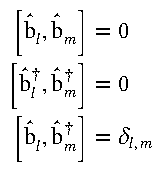
\includegraphics[width=0.5\textwidth]{./main-content/introduction/bosonic-operators.pdf}
            }
        \end{minipage}

        % notes 
        \onslide % on all slides of frame
        \note[item] {
            Wanna discuss, because during the writing of the thesis quite new insight in what in fact the differences of behavior are in between the particle types
        }
        \note[item] {
            First of all wanna point out how we have lattice operators, so fixed sites where there can be particles
        }
        \note[item] {
            Occupation number from 0 to infinity
        }
        \note[item] {
            Nice to handle because they commute
        }
    \end{frame}

    \begin{frame}[t]
        \frametitle{Particle Types}
        
        \vspace{-0.4cm}

        \begin{minipage}[t]{0.5\textwidth}
            \vspace{0pt}
            \begin{itemize}
                \item Bosonic operators
                \begin{itemize}
                    \item Commutation relations
                \end{itemize}
                \item Fermionic operators \pause
                \begin{itemize}
                    \item Anti-commutation relations
                \end{itemize}
            \end{itemize}
        \end{minipage}%
        \onslide
        \hfill
        \begin{minipage}[t]{0.45\textwidth}
            \vspace{0pt}
            \makebox[\textwidth][c]{
                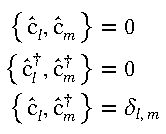
\includegraphics[width=0.5\textwidth]{./main-content/introduction/fermionic-operators.pdf}
            }
        \end{minipage}

        % notes 
        \onslide % on all slides of frame
        \note[item] {
            Occupation number only 0 and one: nice for computational handling
        }
        \note[item] {
            Anti-commute: not so nice to handle in the preparation
        }
    \end{frame}

    \begin{frame}[t]
        \frametitle{Particle Types}
        
        \vspace{-0.4cm}

        \begin{minipage}[t]{0.5\textwidth}
            \vspace{0pt}
            \begin{itemize}
                \item Bosonic operators
                \begin{itemize}
                    \item Commutation relations
                \end{itemize}
                \item Fermionic operators
                \begin{itemize}
                    \item Anti-commutation relations
                \end{itemize}
                \item Hard-core bosonic operators \pause
                \begin{itemize}
                    \item Commutation relations \pause
                    \item Occupation number limited to 0 and 1  \pause
                    \item Number operator is idempotent
                \end{itemize}
            \end{itemize}
        \end{minipage}%
        \onslide
        \hfill
        \begin{minipage}[t]{0.45\textwidth}
            \vspace{0pt}
            \makebox[\textwidth][c]{
                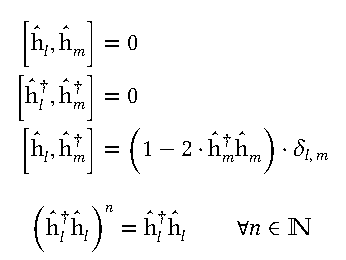
\includegraphics[width=0.85\textwidth]{./main-content/introduction/hard-core-bosonic-operators.pdf}
            }
        \end{minipage}

        % notes 
        \onslide % on all slides of frame
        \note[item] {
            Hard-core bosons: best fo both worlds
        }
        \note[item] {
            Like the fermions nice because only occupation number 0 and 1
        }
        \note[item] {
            but COMMUTATION relations, because of that we will be able to generate an important mapping
        }
        \note[item] {
            Finally: number operator is \emph{idempotent} (power = potenz in english) which we need for one mathematical step later
        }
    \end{frame}

    \begin{frame}[t]
        \frametitle{Particle Types}
        
        \vspace{-0.4cm}

        \begin{minipage}[t]{0.5\textwidth}
            \vspace{0pt}
            \begin{itemize}
                \item Bosonic operators
                \begin{itemize}
                    \item Commutation relations
                \end{itemize}
                \item Fermionic operators
                \begin{itemize}
                    \item Anti-commutation relations
                \end{itemize}
                \item Hard-core bosonic operators
                \begin{itemize}
                    \item Commutation relations
                    \item Occupation number limited to 0 and 1
                    \item Number operator is idempotent
                \end{itemize}
                \item Spins (Pauli operators/matrices)\pause
                \begin{itemize}
                    \item Particles from different sites commute
                    \item Different spin directions on the same site anti-commute
                    \item They obey angular momentum commutation relations
                \end{itemize}
            \end{itemize}
        \end{minipage}%
        \onslide
        \hfill
        \begin{minipage}[t]{0.45\textwidth}
            \vspace{-1.0cm}
            \makebox[\textwidth][c]{
                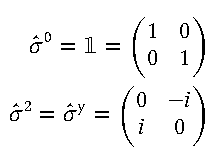
\includegraphics[width=0.55\textwidth,page=1]{./main-content/introduction/spin-operators.pdf}
            }%
            \vspace{-0.3cm}
            \makebox[\textwidth][c]{
                \includegraphics[width=0.55\textwidth,page=2]{./main-content/introduction/spin-operators.pdf}
            }%
            \vspace{-0.1cm}
            \pause[2]
            \makebox[\textwidth][c]{
                \includegraphics[width=0.85\textwidth,page=3]{./main-content/introduction/spin-operators.pdf}
            }
        \end{minipage}

        % notes 
        \onslide % on all slides of frame
        \note[item] {
            Final particle type: spins - watch the 1/2 if it is a pauli or spin operator
        }
        \note[item] {
            Has also mostly commutative properties (also mainly \emph{angular momentum} relations), but also one anti-commutation relation because of the properties of the Pauli matrices
        }
        \note[item] {
            Will be necessary for one mathematical re-formulation
        }
    \end{frame}

    \begin{frame}[t]
        \frametitle{Particle Types - Mappings}
        
        \begin{columns}[t]
            \column{0.4\textwidth}
                \begin{itemize}
                    \item Properties of Pauli matrices \pause
                    \begin{itemize}
                        \item Base of the complex 2x2 matrices \pause
                        \item Can be directly mapped to hard-core bosons
                    \end{itemize}
                \end{itemize}
    
            \onslide
            \column{0.4\textwidth}
                \vspace{-0.5cm}
                \pause[3]
                \makebox[\textwidth][c]{
                    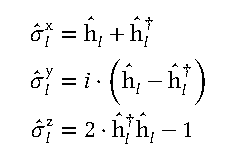
\includegraphics[width=0.6\textwidth,page=1]{./main-content/introduction/transformation.pdf}
                }%
                \vspace{0.1cm}
                \makebox[\textwidth][c]{
                    \includegraphics[width=0.95\textwidth,page=2]{./main-content/introduction/transformation.pdf}
                }
    
        \end{columns}

        % notes 
        \onslide % on all slides of frame
        \note[item] {
            Pauli matrices are a base for the complex 2x2 matrices
        }
        \note[item] {
            Kronecker product of two pauli matrices therefore base for complex 4x4 matrices
        }
        \note[item] {
            Simple transformation that can be verified for its commutation relations or derived from two \emph{Jordan-Wigner Transformations}
        }
        \note[item] {
            Important to watch the order of base states and keep convention or -1 will be introduced unexpectedly
        }
    \end{frame}

    \begin{frame}[t]
        \frametitle{Hamiltonian of the system}
        
        \begin{columns}[t]
            \column{0.4\textwidth}
                \begin{itemize}
                    \item Hubbard model Hamiltonian \pause
                    \item Constant external electric field \pause
                    \item Two particle types (spin degrees) \pause
                    \begin{itemize}
                        \item Different \emph{spins} than for Pauli spin operators
                    \end{itemize}
                \end{itemize}
    
            \onslide
            \column{0.4\textwidth}
                \vspace{-0.0cm}
                \makebox[\textwidth][c]{
                    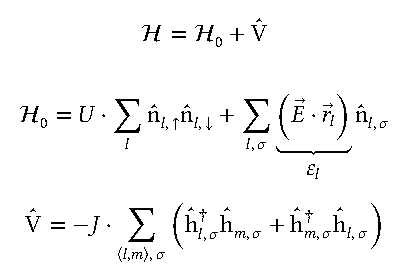
\includegraphics[width=0.95\textwidth,page=1]{./main-content/introduction/hamiltonian.pdf}
                }
    
        \end{columns}

        % notes 
        \onslide % on all slides of frame
        \note[item] {
            Hubbard model:
            \begin{itemize}
                \item Double occupation term
                \item Two particle degrees of freedom (= spin but not same spin as before: so also written as h and d)
                \item Here: electrical field that acts symmetrical on both spin directions
                \item Hopping term that is here treated as a perturbation 
            \end{itemize}
        }
    \end{frame}

    \begin{frame}[t]
        \frametitle{Geometry of the system}
        
        \begin{columns}[t]
            \column{0.4\textwidth}
                \begin{itemize}
                    \item 2-dimensional geometry \pause
                    \item Square lattice arrangement \pause
                    \item Computation for general size and field angle
                \end{itemize}
    
            \onslide
            \column{0.4\textwidth}
                \vspace{0.0cm}
                \makebox[\textwidth][c]{
                    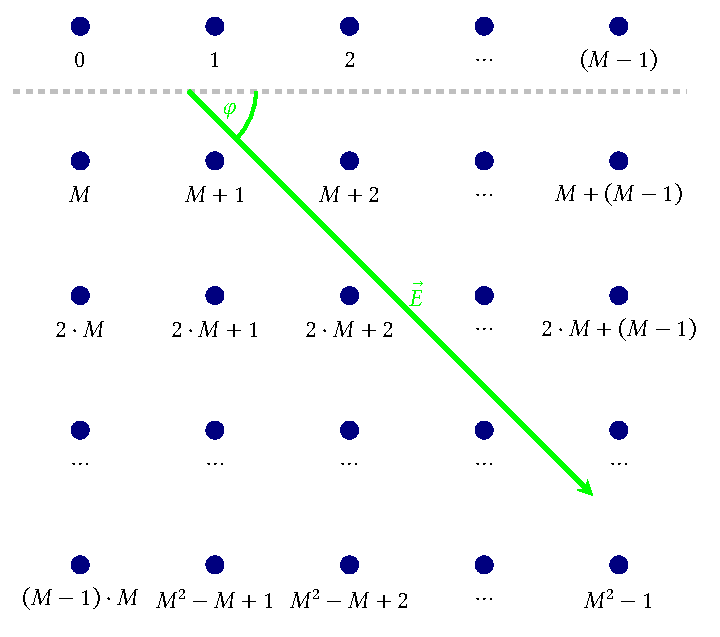
\includegraphics[width=1.0\textwidth,page=1]{./main-content/introduction/geometry.pdf}
                }
    
        \end{columns}

        % notes 
        \onslide % on all slides of frame
        \note[item] {
            two-dimensional
        }
        \note[item] {
            square
        }
        \note[item] {
            Electrical field and we want to calculate generally for angle, field strength and number of sites
        }
    \end{frame}